\documentclass{article} 
\usepackage[a4paper]{geometry} 
\usepackage{graphicx} 
\usepackage{hyperref} 
\usepackage{amsmath,amssymb} 
\usepackage{caption} 
\usepackage{subcaption}
\usepackage{pdflscape}

\title{Tevatron Higgs} 
\author{ Daniel C E Bunting \& Amalia Madden} 
\date{\today}

\begin{document}

\maketitle
\begin{abstract}
\end{abstract}

\section{Introduction} % (fold)
\label{sec:introduction}

% section introduction (end)

\section{Theory} % (fold)
\label{sec:theory}



% section theory (end)


\section{Method} % (fold)
\label{sec:method}

\subsection{Feature Selection} % (fold)
\label{sub:feature_selection}
%!TEX root = /Users/Daniel/Documents/Imperial/project/tevatron-higgs/report/report.tex

In any scenario where statistical methods are used to interpret data selecting features in order to maximise the discriminatory or explanatory power of the model plays a critical role.
From the b-tagged jets, those with the highest and second highest transverse momentum $P_t$ were identified as being the putative product of the decaying Higgs boson, with all the following variable differences are considered to be taken between these leading jets. 
Following \cite{Abazov201197} seven feature variables were extracted from the raw simulation data, and used as inputs to the classification neural network. 

\subsubsection*{Pseudorapidity difference $ \Delta\eta $ } % (fold)
\label{ssub:pseudorapidity}

Te pseudorapidity of a jet is defined as
\begin{equation}
	\eta = - \ln\left[\tan\left( \frac{\theta}{2} \right)\right]
\end{equation}
where $\theta$ is the angle between the jet and the beam axis. The pseudorapidity is preferred to $\theta$ as the difference between two pseudorapidity is Lorentz invariant.
% subsubsection pseudorapidity (end)


\subsubsection*{Momentum balance $P_{balance}$} % (fold)
\label{ssub:momentum_balance_p__balance}

The momentum balance of the leading b jet pair is defined

\begin{equation}
	P_{balance} = \frac{\left|p_1 - p_2\right|}{ \left|p_1 + p_2\right|}  
\end{equation}

% subsubsection momentum_balance_p__balance (end)

\subsubsection*{Sphericity $S$} % (fold)
\label{ssub:sphericity_s}
	The sphericity is defined as 
	\begin{equation}
		S = \frac{3}{2} (\lambda_2 + \lambda_3)
	\end{equation}

	where $\lambda_2$ and $\lambda_3$ are the second and third largest eigenvalues of the sphericity tensor $\mathbf{\hat{S}}^{\alpha\beta}$
	\begin{equation}
		\mathbf{\hat{S}}^{\alpha\beta} = \frac{\sum_i p_{\alpha}^i p_{\beta}^i}{\sum_i |p^i|^2}
	\end{equation}

% subsubsection sphericity_s (end)

\subsubsection{Invariant Mass} % (fold)
\label{ssub:invariant_mass}

\begin{equation}
	M_H = \sqrt{\sum_{Dijet}{E^2 - p^2}}
\end{equation}

As can be seen in Table~\ref{tab:corr} the invariant dijet mass is a strong predictor of whether an event is Higgs decay and including it in the ANN significantly increased its discriminatory power.
However since the Higgs mass is not predicted by the Standard Model it must be hypothesised during the simulation stage, so in order to avoid training the ANN to depend too heavily on a particular value of $M_H$ we tested models both with and without $M_H$
% subsubsection invariant_mass (end)


Additionally we define the \textbf{azimuthal angle difference $ \Delta\phi $}, the \textbf{combined pseudorapidity $\eta_H$}, the \textbf{difference between the leading jet and the Higgs $\eta_H - \eta_1$}.

\begin{figure}[htbp]
	\centering
	\begin{subfigure}[b]{0.395\textwidth}
		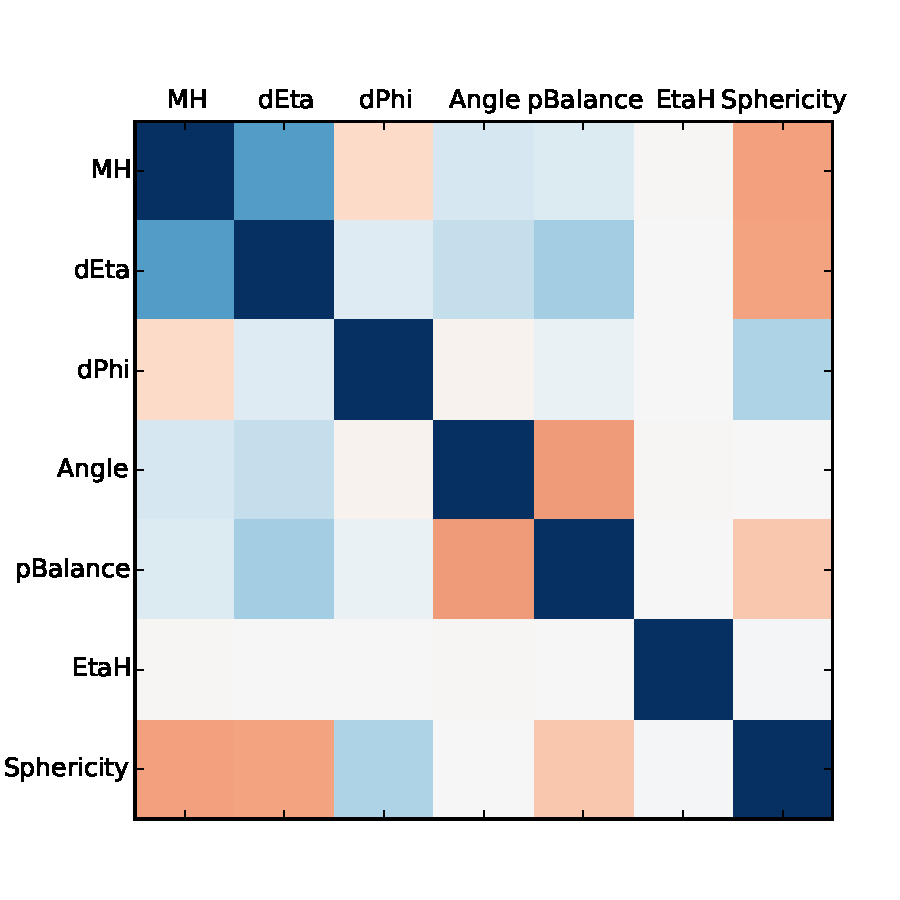
\includegraphics[width=\textwidth]{img/background_corr}
		\caption{Background}
		\label{fig:mh}
		\vspace{7mm}
	\end{subfigure}
	\begin{subfigure}[b]{0.5\textwidth}
		                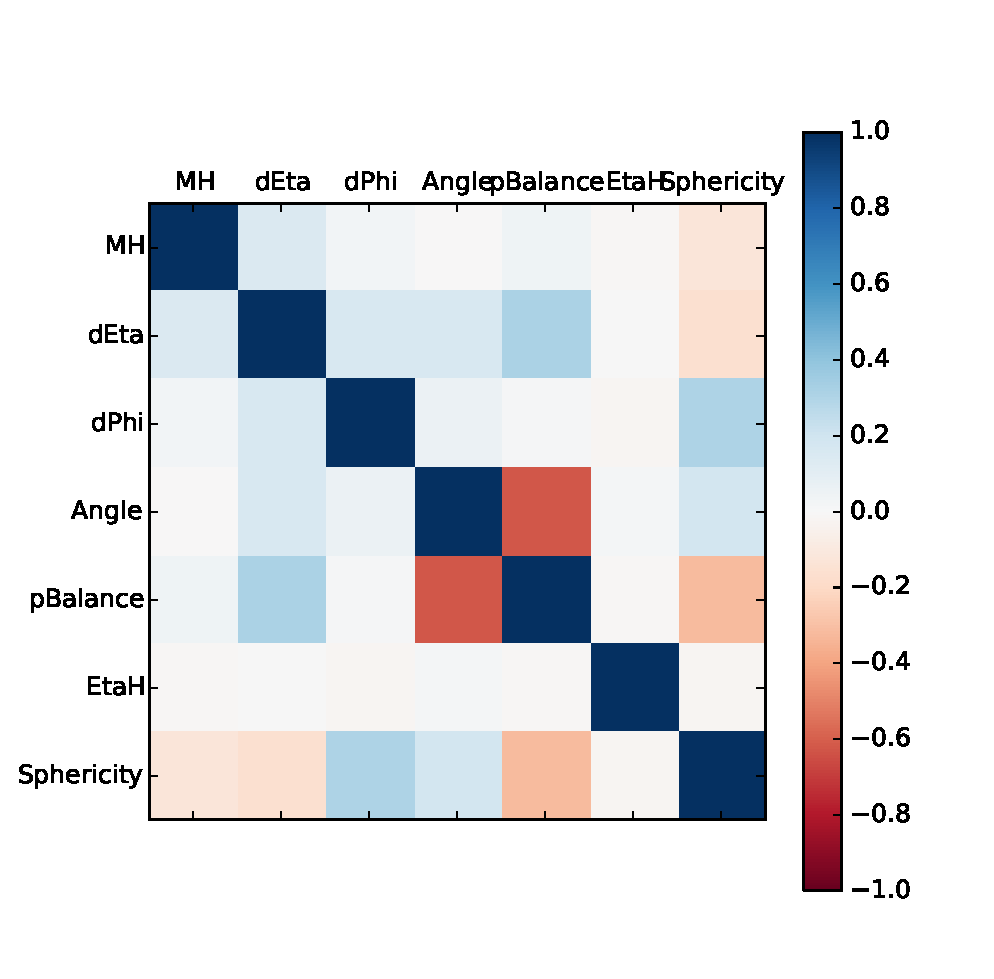
\includegraphics[width=\textwidth]{img/signal_corr}
		                \caption{Signal}
		                \label{fig:mh}
		\end{subfigure}
	
	\caption{Matrices of the Pearson product-moment correlation coefficients between each of the features}
	\label{fig:cormat}
	\end{figure} 

	
In order to evaluate the the feature selection the correlation matrices between the features for the signal and background events were calculated and shown in Figure~\ref{fig:cormat}. 
The correlations between each feature and the output variable were also calculated and are summarised in  Table~\ref{tab:corr}. 
The features selected for inclusion in a model should be both highly correlated with the output and weakly correlated with each other. A high correlation between two features suggests redundancy, which should be avoided as unnecessarily complex models take longer and require more data (which may not be available) to train.
$\eta_{H}$ is a potential candidate for removal since it is very weakly correlated with the output.  
	\begin{table}
		\begin{center}
		\begin{tabular}{ll}
			\textbf{Feature} & \textbf{Correlation} \\
			\hline
			$\Delta\eta$ & 0.329\\			
			$M_{H}$ & 0.204 \\
			$\Delta\Phi$ &  0.176\\
			Sphericity & 0.150\\
			Momentum Balance &  0.134\\
			$\eta_H - \eta_1$ &  0.0343 \\
			$\eta_{H}$ & 0.00359\\
			
		\end{tabular}
		\end{center}
		\caption{The correlation between each of the features and the output variable}
		\label{tab:corr}
	\end{table}
	

\begin{figure}[htbp]
	\centering	
	\begin{subfigure}[b]{0.3\textwidth}
	                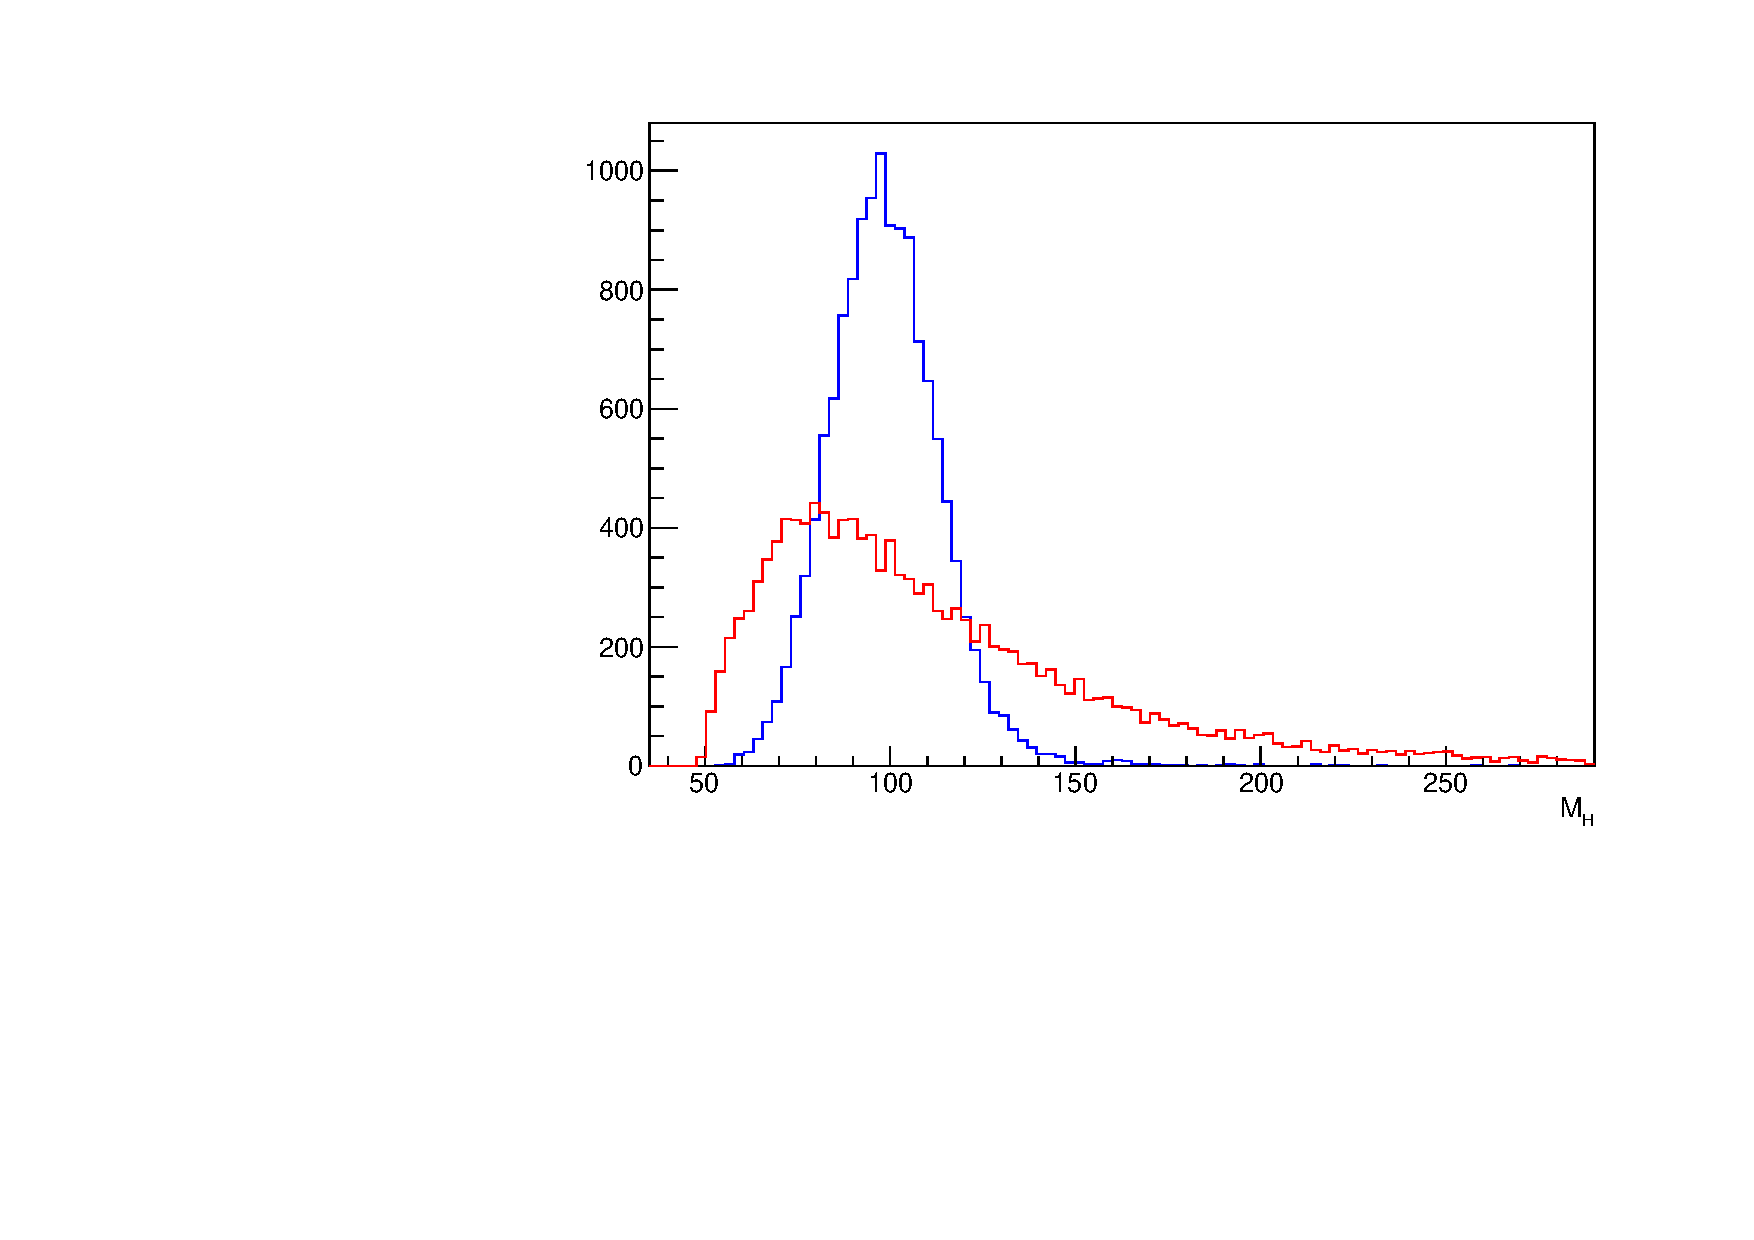
\includegraphics[width=\textwidth]{img/mh}
	                \caption{Invariant mass}
	                \label{fig:mh}
	\end{subfigure}
	\begin{subfigure}[b]{0.3\textwidth}
	                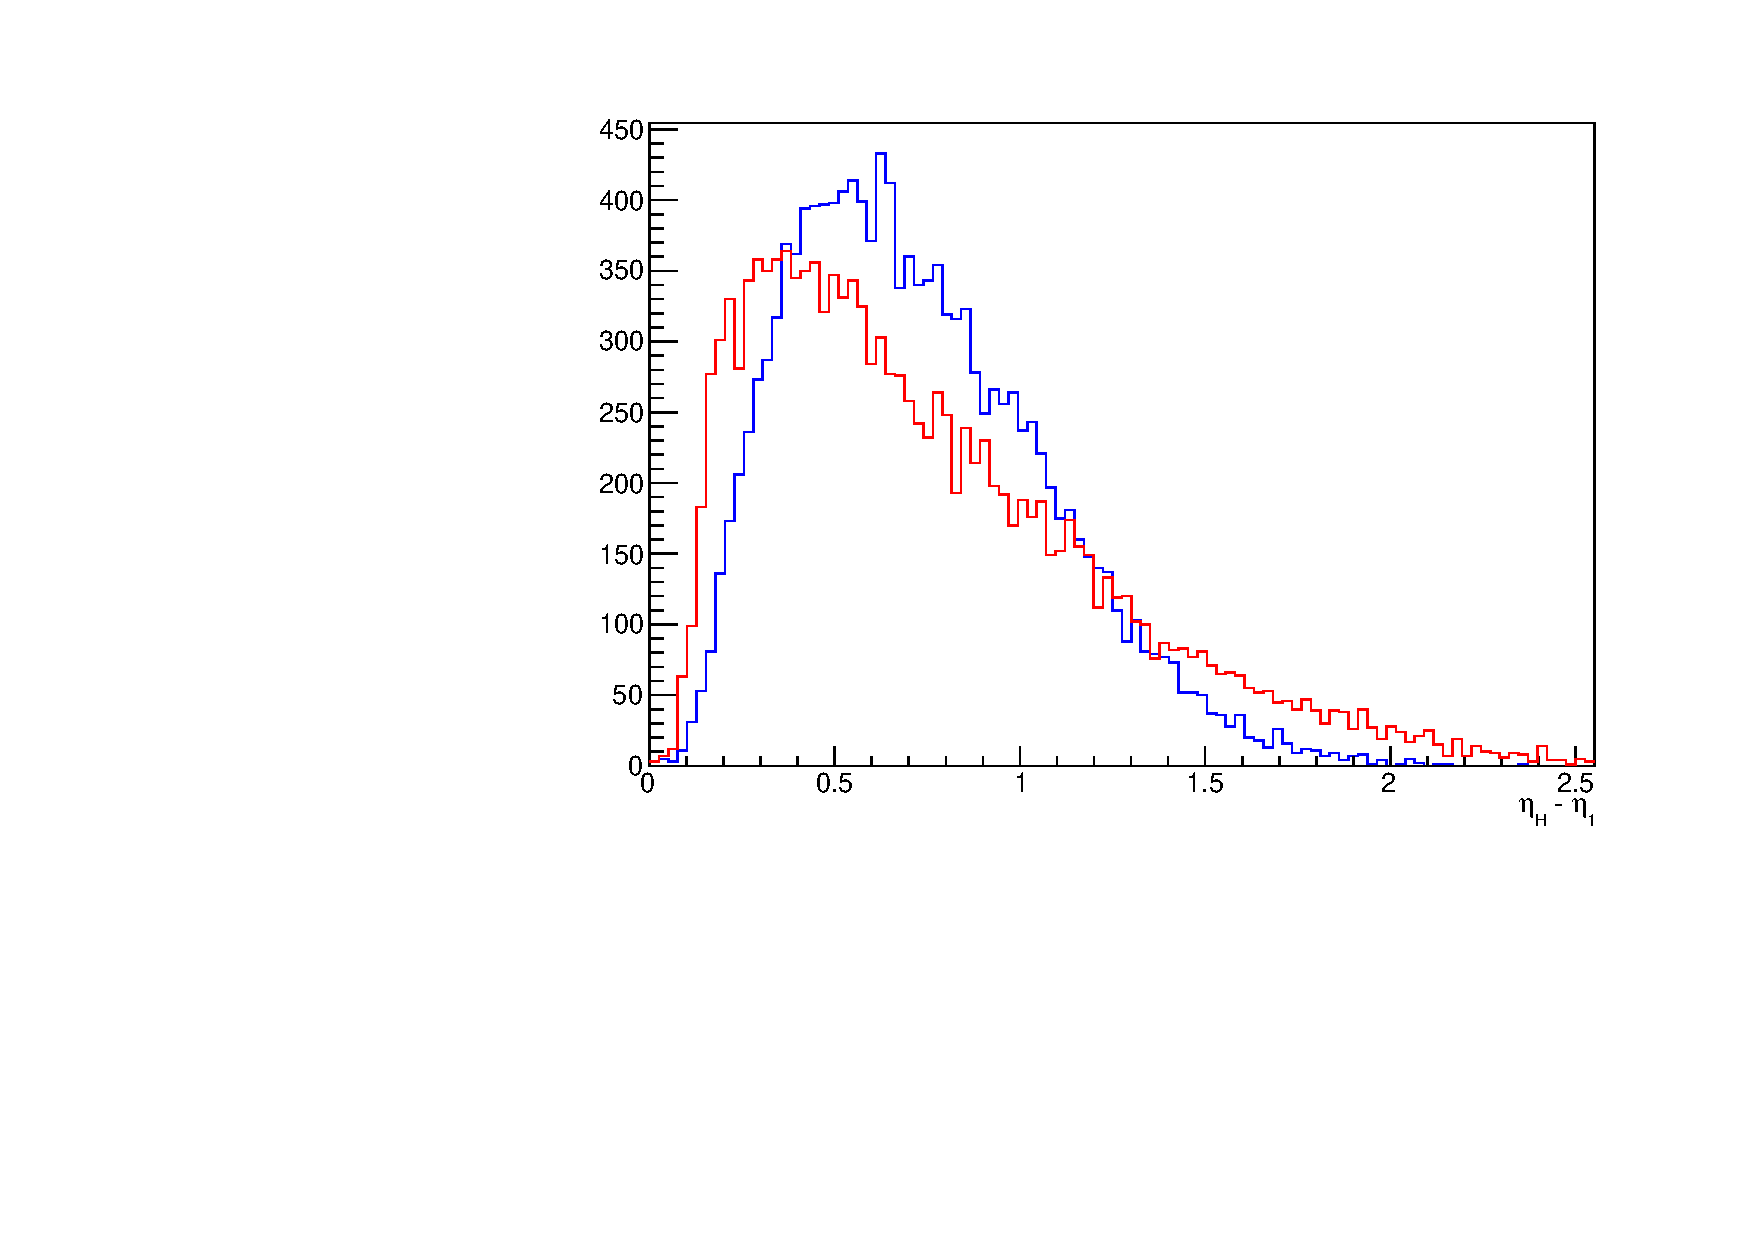
\includegraphics[width=\textwidth]{img/angle}
	                \caption{$\eta_H - \eta_1$}
	                \label{fig:angle}
	\end{subfigure}
	\begin{subfigure}[b]{0.3\textwidth}
	                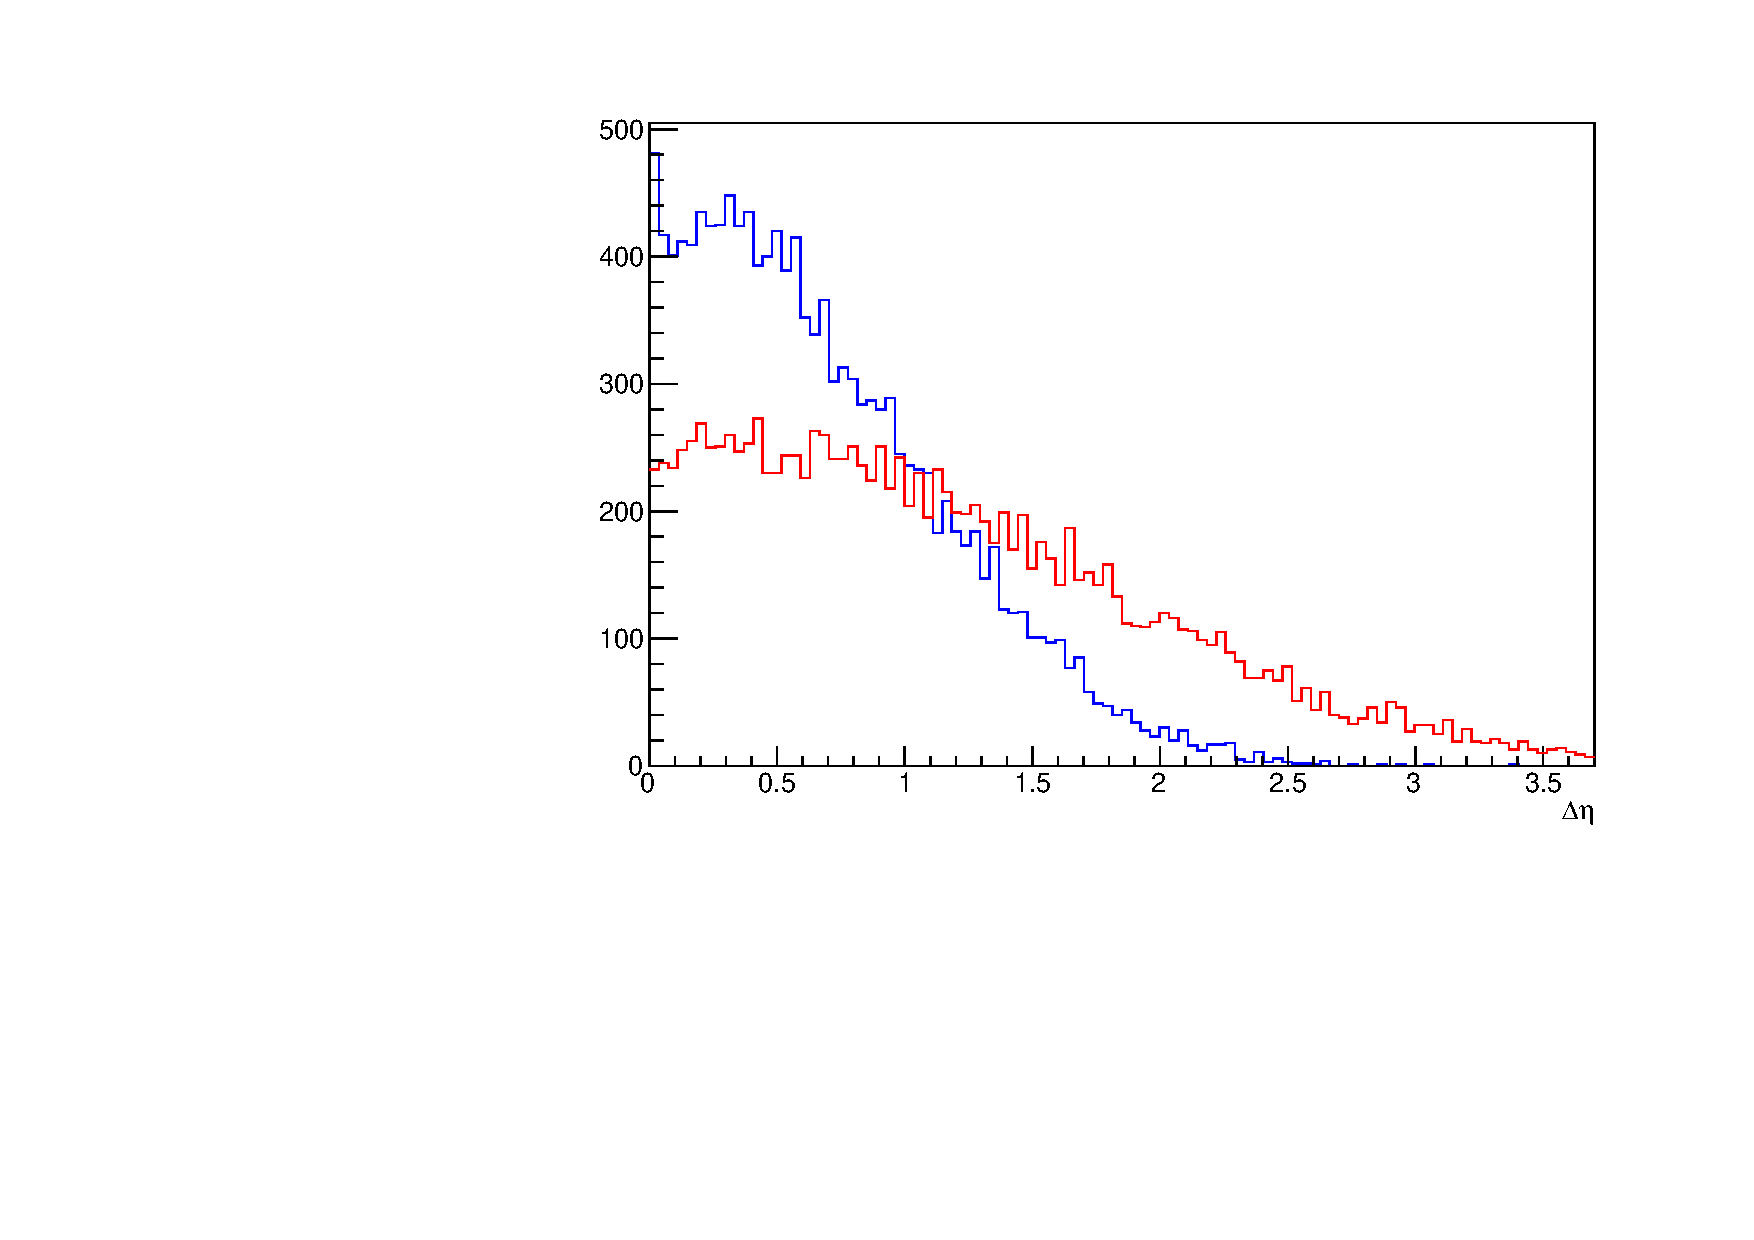
\includegraphics[width=\textwidth]{img/deta}
	                \caption{$\Delta\eta$}
	                \label{fig:deta}
	\end{subfigure}
	\begin{subfigure}[b]{0.3\textwidth}
	                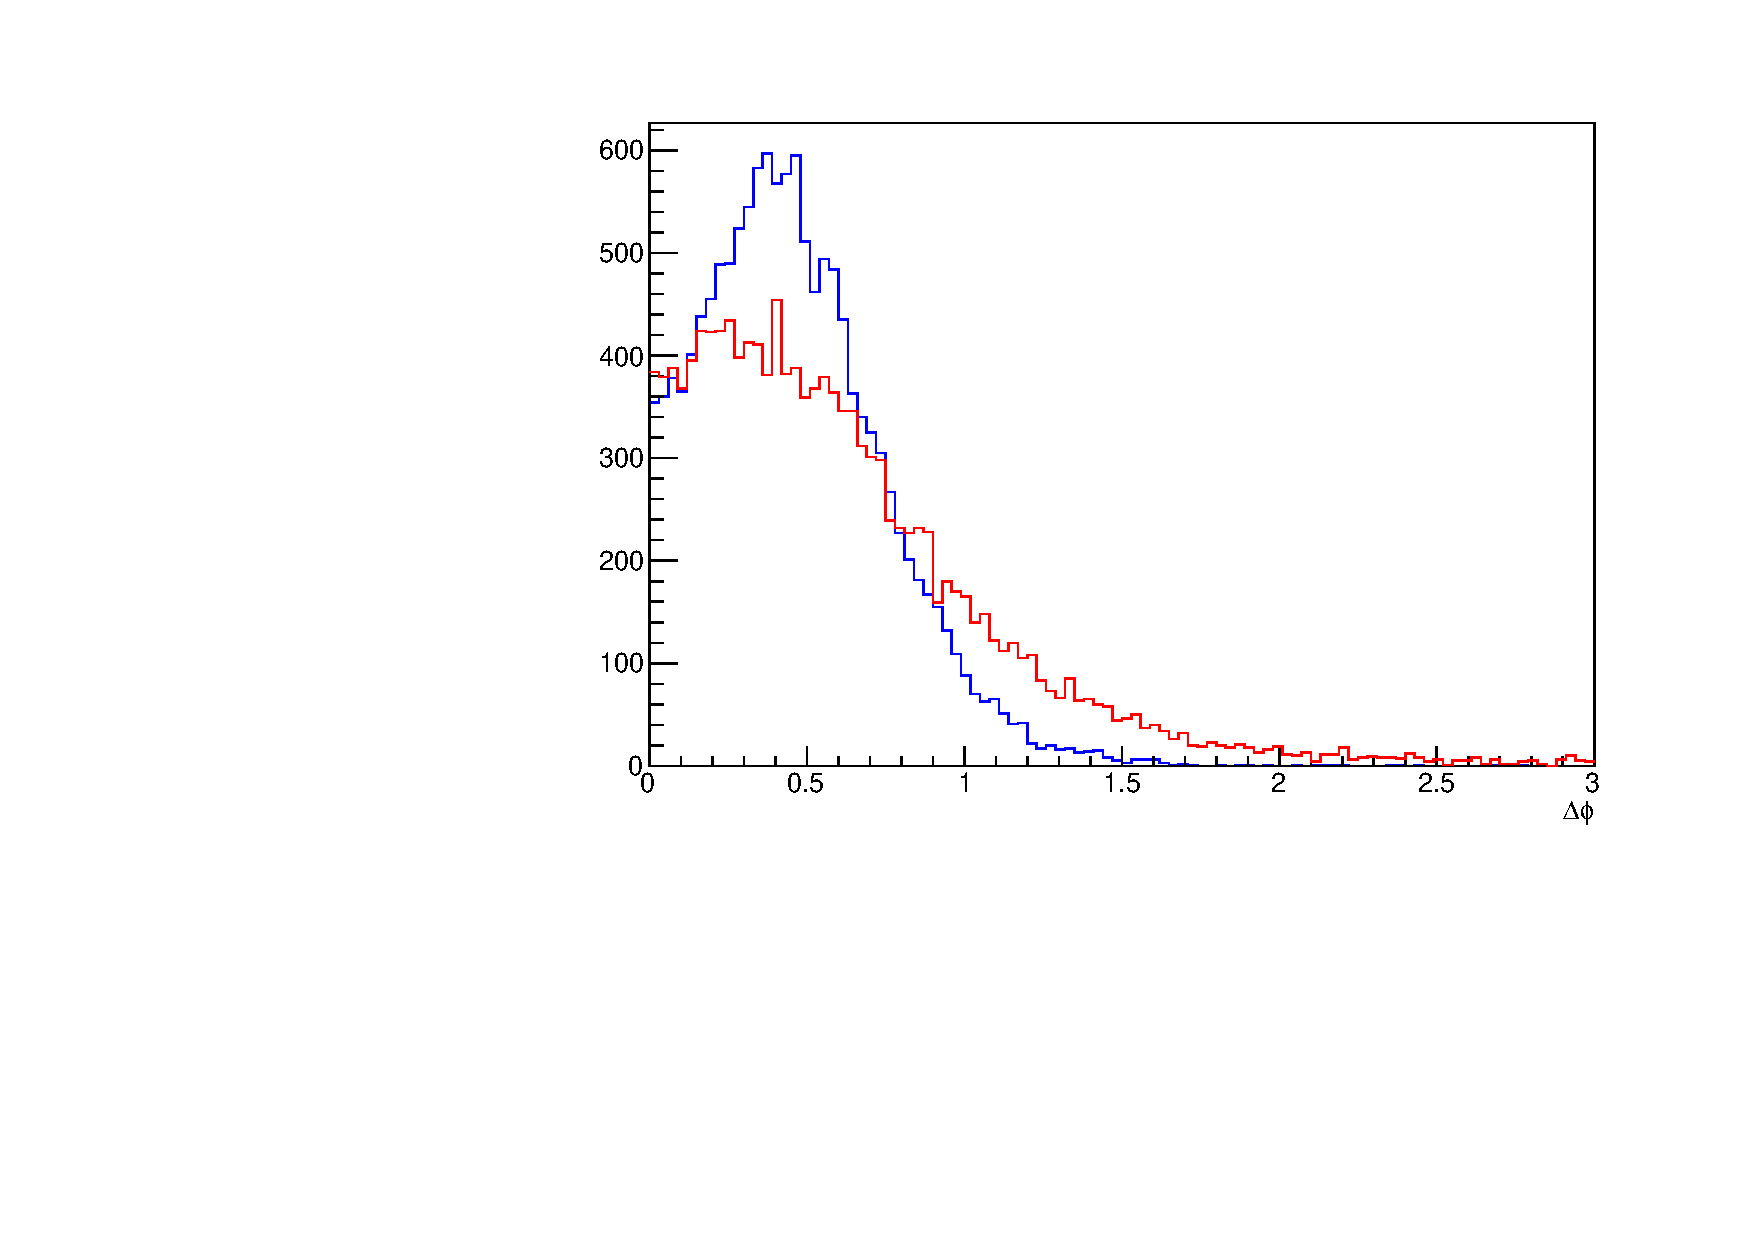
\includegraphics[width=\textwidth]{img/dphi}
	                \caption{$\Delta\phi$}
	                \label{fig:dphi}
	\end{subfigure}	
	\begin{subfigure}[b]{0.3\textwidth}
	                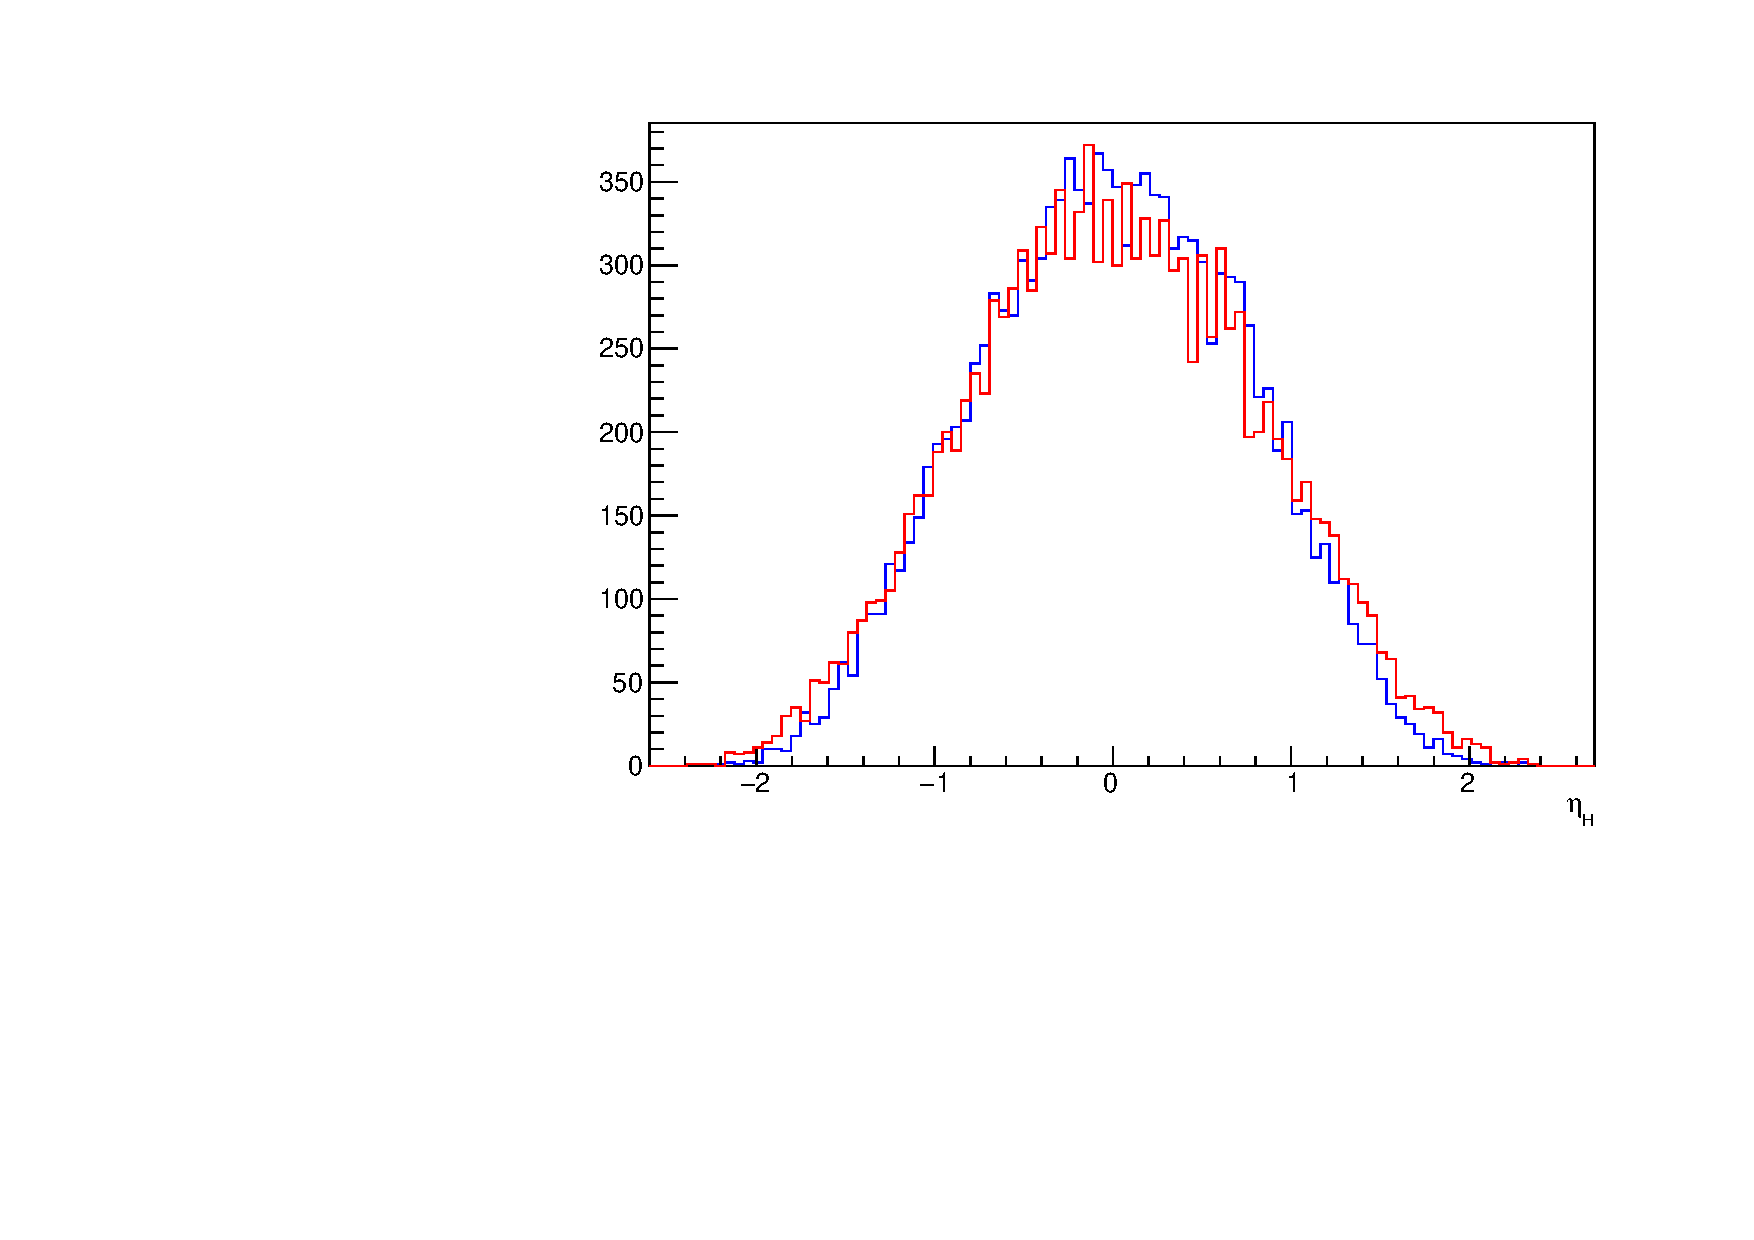
\includegraphics[width=\textwidth]{img/etah}
	                \caption{$\eta_H$}
	                \label{fig:etah}
	\end{subfigure}
	\begin{subfigure}[b]{0.3\textwidth}
	                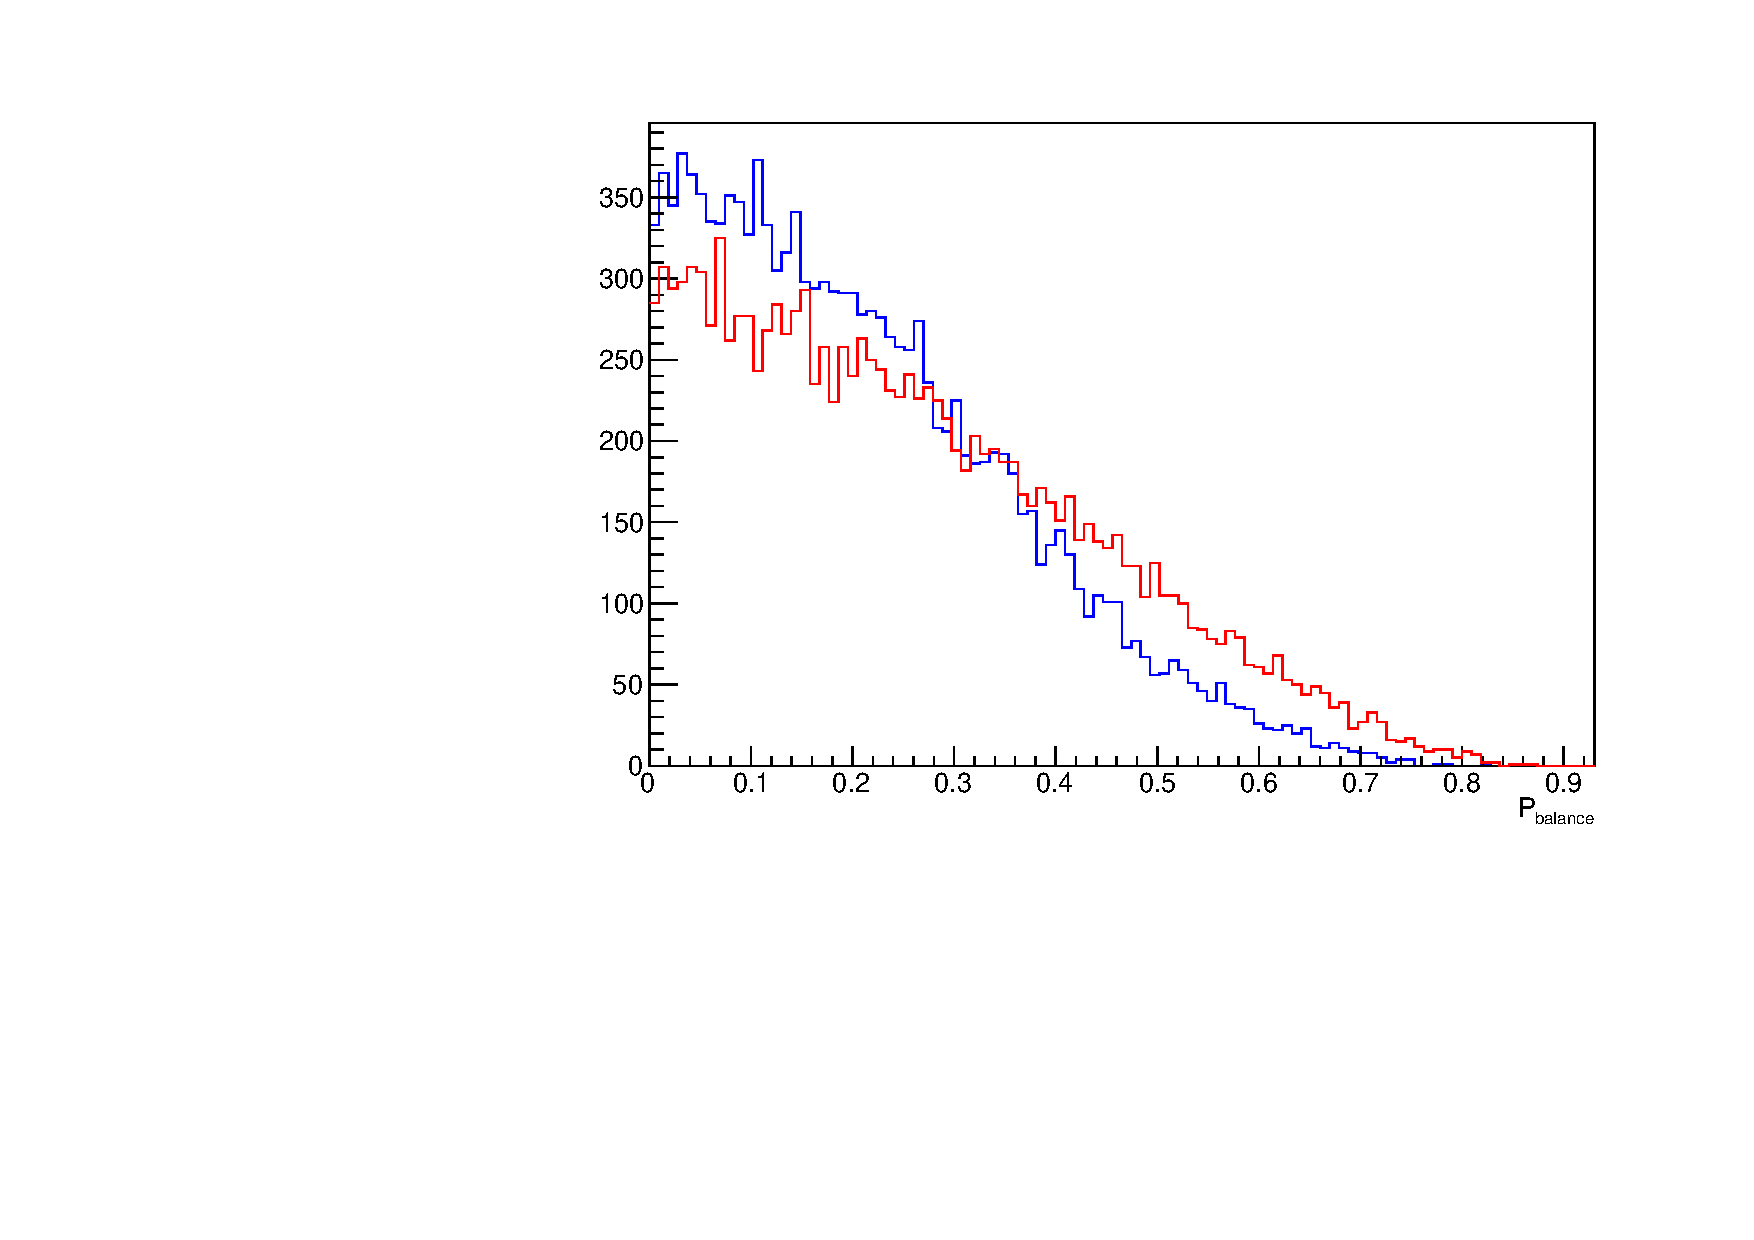
\includegraphics[width=\textwidth]{img/pbalance}
	                \caption{Momentum balance}
	                \label{fig:pbal}
	\end{subfigure}
	\begin{subfigure}[b]{0.3\textwidth}
	                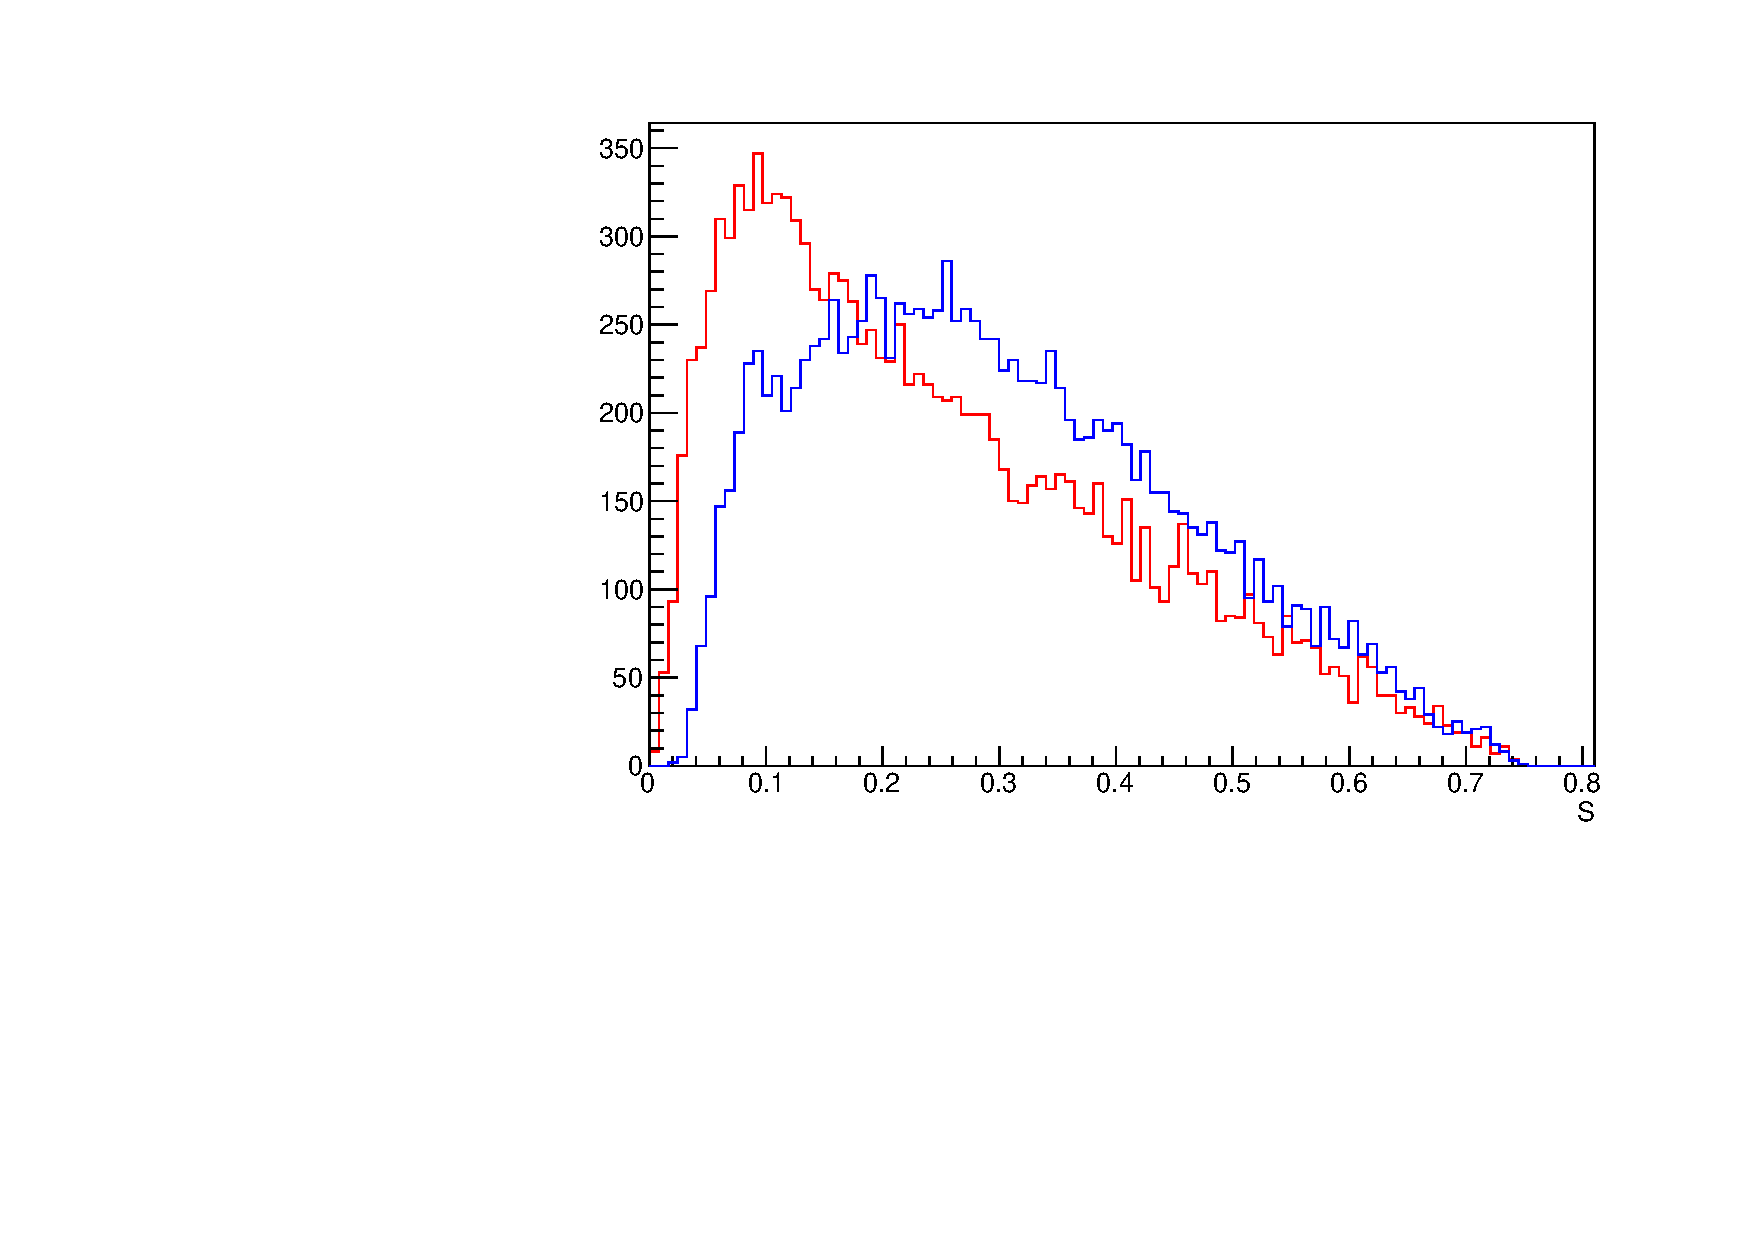
\includegraphics[width=\textwidth]{img/sphericity}
	                \caption{Sphericity}
	                \label{fig:sphericity}
	\end{subfigure}

	\caption{Distributions of the input features. All y scales are events. The signal is in blue and the background in red.}
	
	\label{fig:label}



\end{figure}


% subsection feature_selection (end)
\subsection{Artificial Neural Networks} % (fold)
\label{sub:artificial_neural_networks}


Heloo this is a test
% subsection artificial_neural_networks (end)

% section method (end)

\section{Discusion} % (fold)
\label{sec:discusion}

% section discusion (end)

\section{Conclusion} % (fold)
\label{sec:conclusion}

% section conclusion (end)




\bibliography{tevatronhiggs}
\bibliographystyle{unsrt} 

\clearpage

\end{document} 
